\section{Data Type}

\begin{frame}
  \frametitle{Chisel Type}

  Chisel Type is abstract data type for Verilog.

  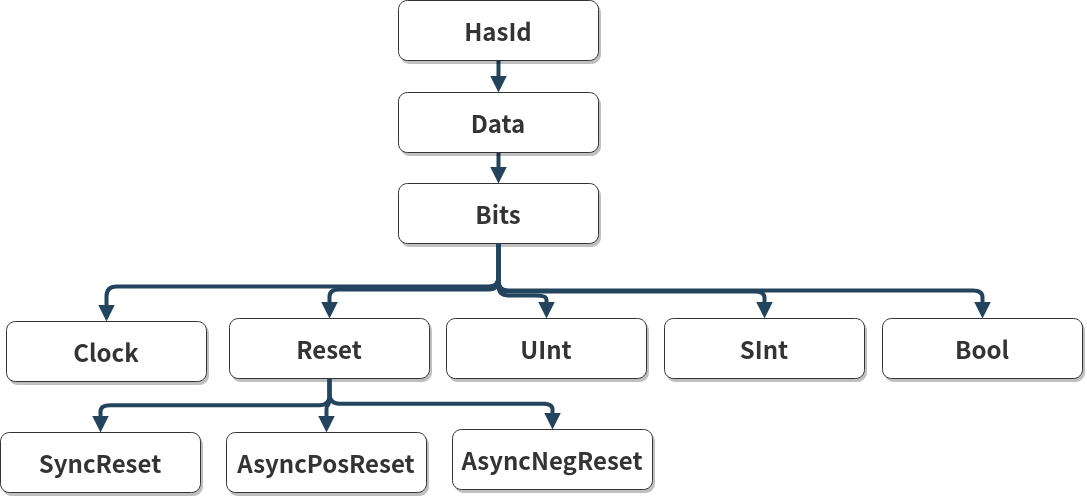
\includegraphics[width = 12cm]{./fig/datatype.png}
\end{frame}

\begin{frame}
  \frametitle{Hardware Type}

  Bind \Emph{Chisel Type} to \emph{Synthesizable} Verilog Type:

  \begin{block}{Constrained Binding}
    Used for connection, care about which module scope.
    \begin{itemize}
      \item OpBinding (read only)
      \item PortBinding
      \item RegBinding
      \item WireBinding
    \end{itemize}
  \end{block}

  \begin{block}{Unconstrained Binding}
    Not for connection, don't care about which module scope.
    \begin{itemize}
    \item LitBinding
    \end{itemize}
  \end{block}

\end{frame}

\begin{frame}
  \frametitle{Bits}

  \begin{itemize}
    \item Suggest Name: User specified
    \item Reference: associate with IR
    \item Binding: is Synthesizable
    \item Type: IR Type
    \item Direction: Input/Output/InOut
    \item Op Methods: +/-/\&/~ ...
  \end{itemize}

\end{frame}
